
\section{Data to Monte Carlo comparison requiring at least 1 \bjet}
\label{app:datamc1tagin}



\subsection{Electron channel}

\begin{figure}[h!]\begin{center}
	\subfigure[]{
  	\includegraphics[width=0.29\textwidth]{vlq_analysis/figures/THESIS_c5_presel_noortho_noyields/ELE/4jetin/1btagin/Njets25_ELE_4jetin1btagin_NOMINAL}}
	\subfigure[]{
  	\includegraphics[width=0.29\textwidth]{vlq_analysis/figures/THESIS_c5_presel_noortho_noyields/ELE/4jetin/1btagin/JetPt1_ELE_4jetin1btagin_NOMINAL}}
	\subfigure[]{
  	\includegraphics[width=0.29\textwidth]{vlq_analysis/figures/THESIS_c5_presel_noortho_noyields/ELE/4jetin/1btagin/JetEta1_ELE_4jetin1btagin_NOMINAL}}\\
	\subfigure[]{
  	\includegraphics[width=0.29\textwidth]{vlq_analysis/figures/THESIS_c5_presel_noortho_noyields/ELE/4jetin/1btagin/MET_ELE_4jetin1btagin_NOMINAL}}
	\subfigure[]{
  	\includegraphics[width=0.29\textwidth]{vlq_analysis/figures/THESIS_c5_presel_noortho_noyields/ELE/4jetin/1btagin/LepPt_ELE_4jetin1btagin_NOMINAL}}
	\subfigure[]{
  	\includegraphics[width=0.29\textwidth]{vlq_analysis/figures/THESIS_c5_presel_noortho_noyields/ELE/4jetin/1btagin/LepEta_ELE_4jetin1btagin_NOMINAL}}\\
	\subfigure[]{
  	\includegraphics[width=0.29\textwidth]{vlq_analysis/figures/THESIS_c5_presel_noortho_noyields/ELE/4jetin/1btagin/Wlep_MassT_ELE_4jetin1btagin_NOMINAL}}
	\subfigure[]{
  	\includegraphics[width=0.29\textwidth]{vlq_analysis/figures/THESIS_c5_presel_noortho_noyields/ELE/4jetin/1btagin/HTHad_ELE_4jetin1btagin_NOMINAL}}
	\subfigure[]{
  	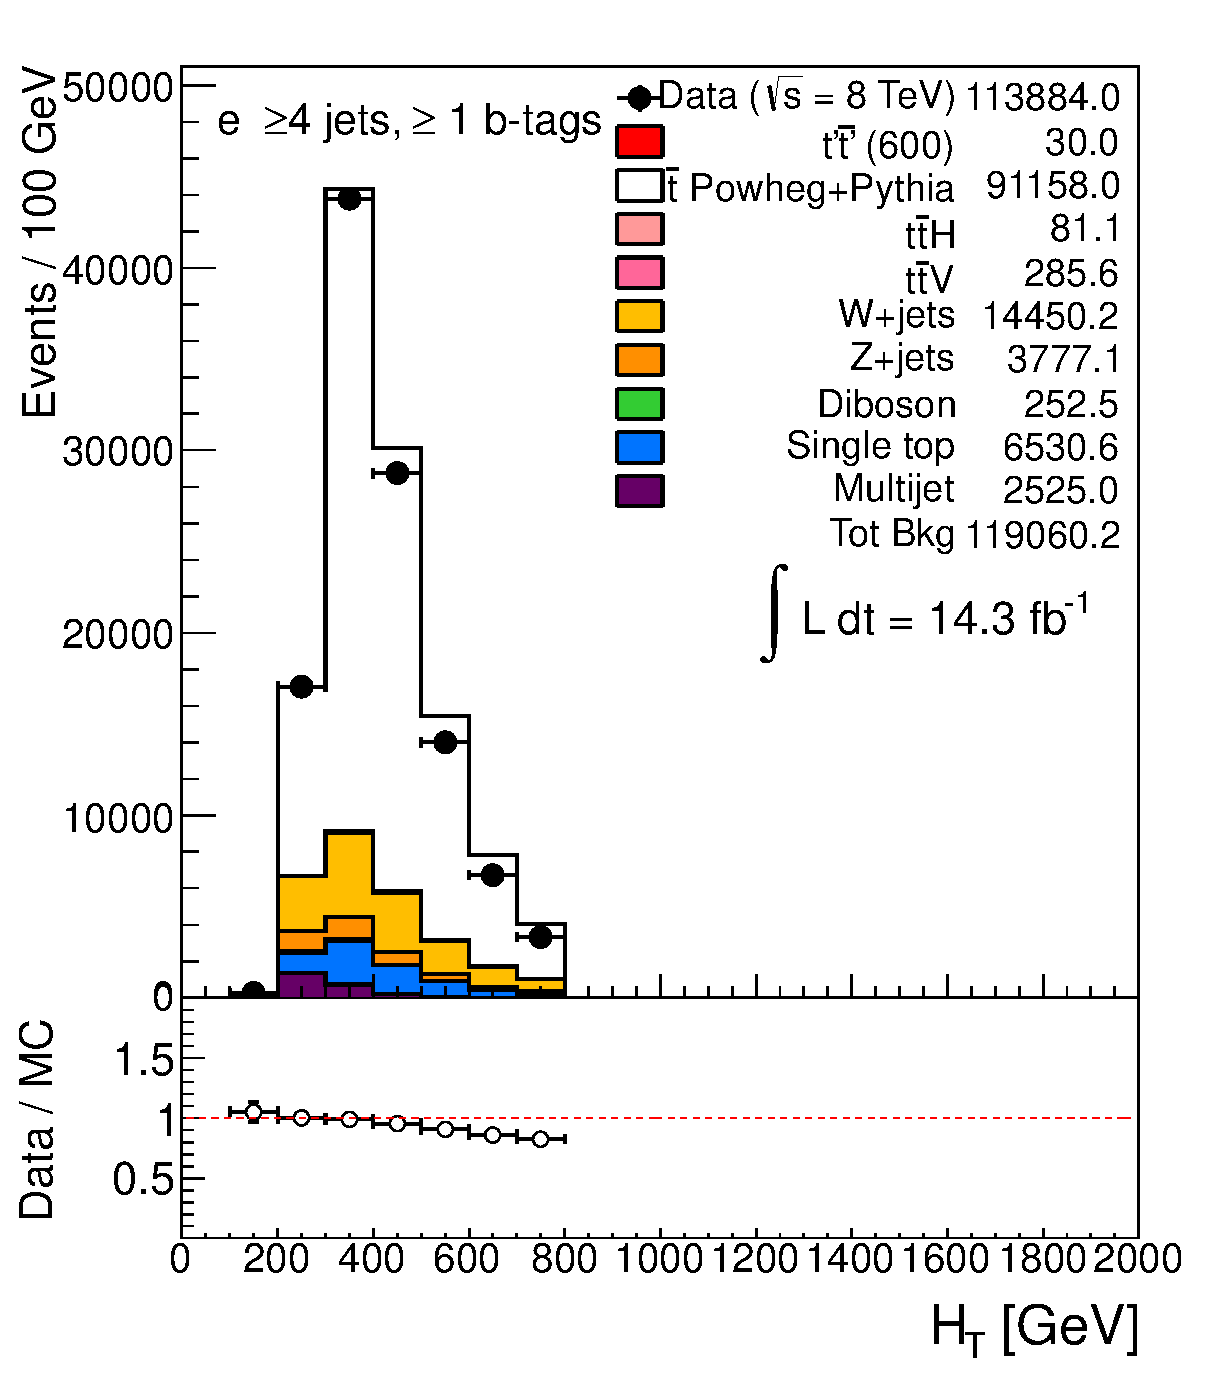
\includegraphics[width=0.29\textwidth]{vlq_analysis/figures/THESIS_c5_presel_noortho_noyields/ELE/4jetin/1btagin/HTAll_ELE_4jetin1btagin_NOMINAL}}
	\caption[]{Comparison between data and prediction in the
        electron
        channel in the blinded control region with at least four jets and
        no \bjet s
        \input{appendices/datamc_variablelist.tex}
         \label{fig:appELE_4jetin1btagin}}
\end{center}\end{figure}


\clearpage
\subsection{Muon channel}


\begin{figure}[h!]\begin{center}
	\subfigure[]{
  	\includegraphics[width=0.29\textwidth]{vlq_analysis/figures/THESIS_c5_presel_noortho_noyields/MUON/4jetin/1btagin/Njets25_MUON_4jetin1btagin_NOMINAL}}
	\subfigure[]{
  	\includegraphics[width=0.29\textwidth]{vlq_analysis/figures/THESIS_c5_presel_noortho_noyields/MUON/4jetin/1btagin/JetPt1_MUON_4jetin1btagin_NOMINAL}}
	\subfigure[]{
  	\includegraphics[width=0.29\textwidth]{vlq_analysis/figures/THESIS_c5_presel_noortho_noyields/MUON/4jetin/1btagin/JetEta1_MUON_4jetin1btagin_NOMINAL}}\\
	\subfigure[]{
  	\includegraphics[width=0.29\textwidth]{vlq_analysis/figures/THESIS_c5_presel_noortho_noyields/MUON/4jetin/1btagin/MET_MUON_4jetin1btagin_NOMINAL}}
	\subfigure[]{
  	\includegraphics[width=0.29\textwidth]{vlq_analysis/figures/THESIS_c5_presel_noortho_noyields/MUON/4jetin/1btagin/LepPt_MUON_4jetin1btagin_NOMINAL}}
	\subfigure[]{
  	\includegraphics[width=0.29\textwidth]{vlq_analysis/figures/THESIS_c5_presel_noortho_noyields/MUON/4jetin/1btagin/LepEta_MUON_4jetin1btagin_NOMINAL}}\\
	\subfigure[]{
  	\includegraphics[width=0.29\textwidth]{vlq_analysis/figures/THESIS_c5_presel_noortho_noyields/MUON/4jetin/1btagin/Wlep_MassT_MUON_4jetin1btagin_NOMINAL}}
	\subfigure[]{
  	\includegraphics[width=0.29\textwidth]{vlq_analysis/figures/THESIS_c5_presel_noortho_noyields/MUON/4jetin/1btagin/HTHad_MUON_4jetin1btagin_NOMINAL}}
	\subfigure[]{
  	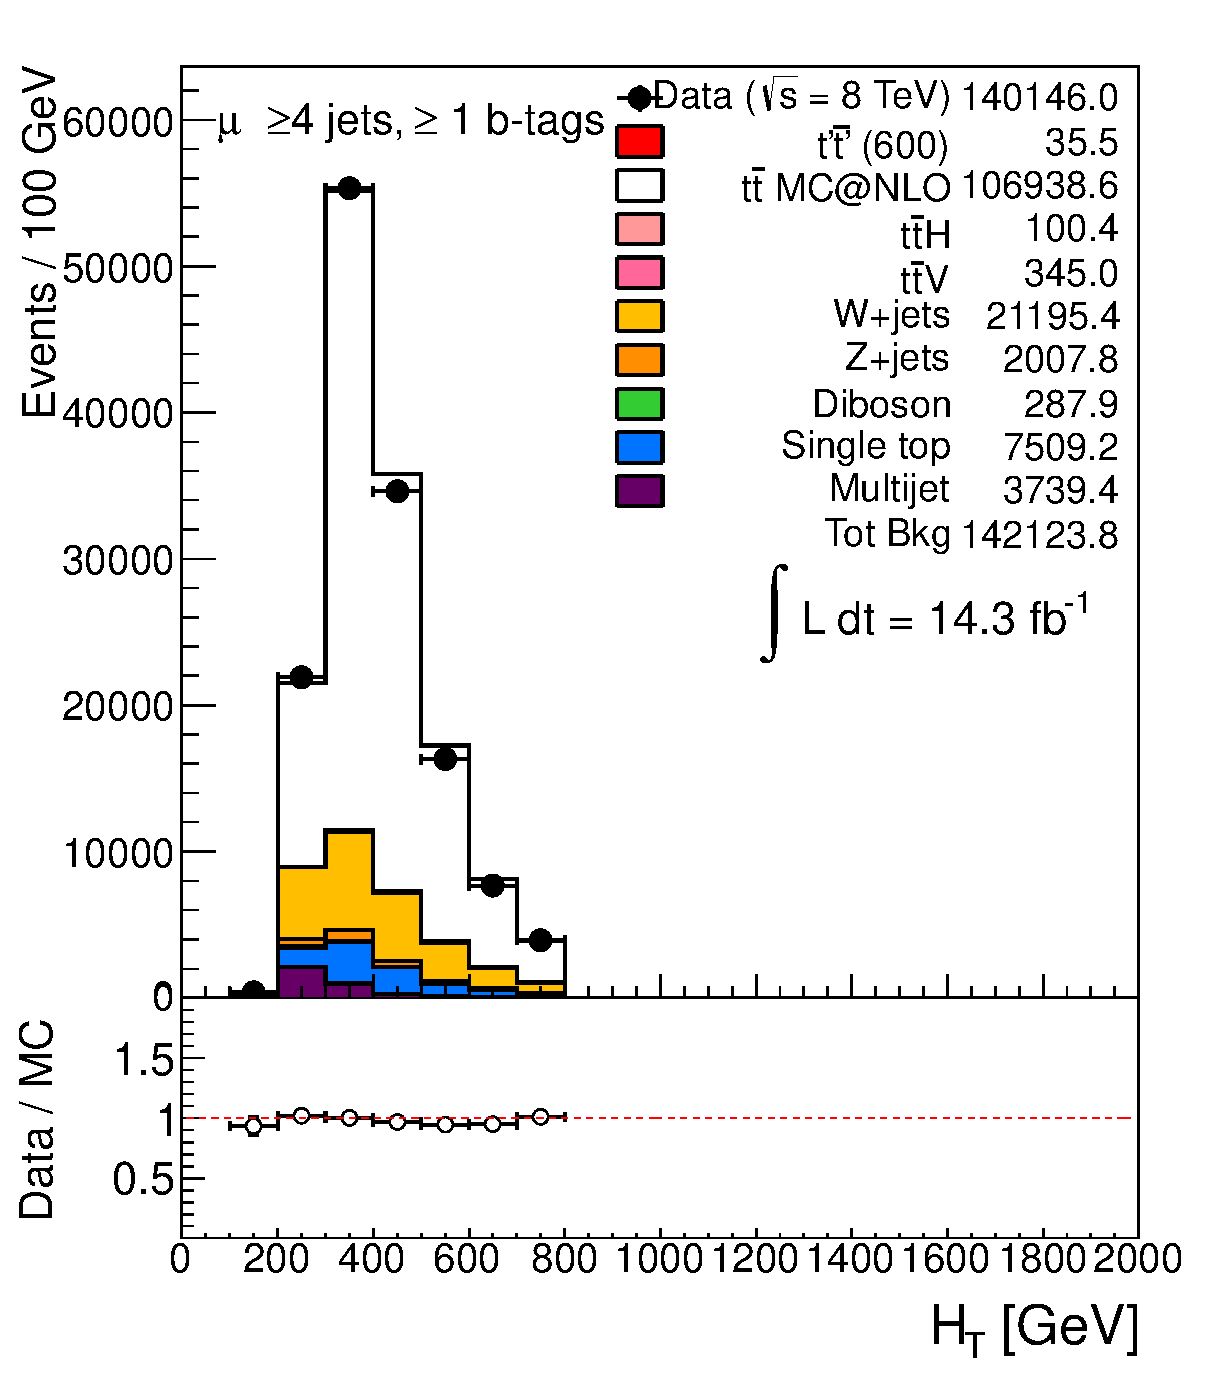
\includegraphics[width=0.29\textwidth]{vlq_analysis/figures/THESIS_c5_presel_noortho_noyields/MUON/4jetin/1btagin/HTAll_MUON_4jetin1btagin_NOMINAL}}
	\caption[]{Comparison between data and prediction in the
        muon 
        channel in the blinded control region with at least four jets and
        no \bjet s
        \input{appendices/datamc_variablelist.tex}
	\label{fig:appMUON_4jetin1btagin}}
\end{center}\end{figure}


\clearpage
\subsection{Electron+Muon channel}

\begin{figure}[h!]\begin{center}
	\subfigure[]{
  	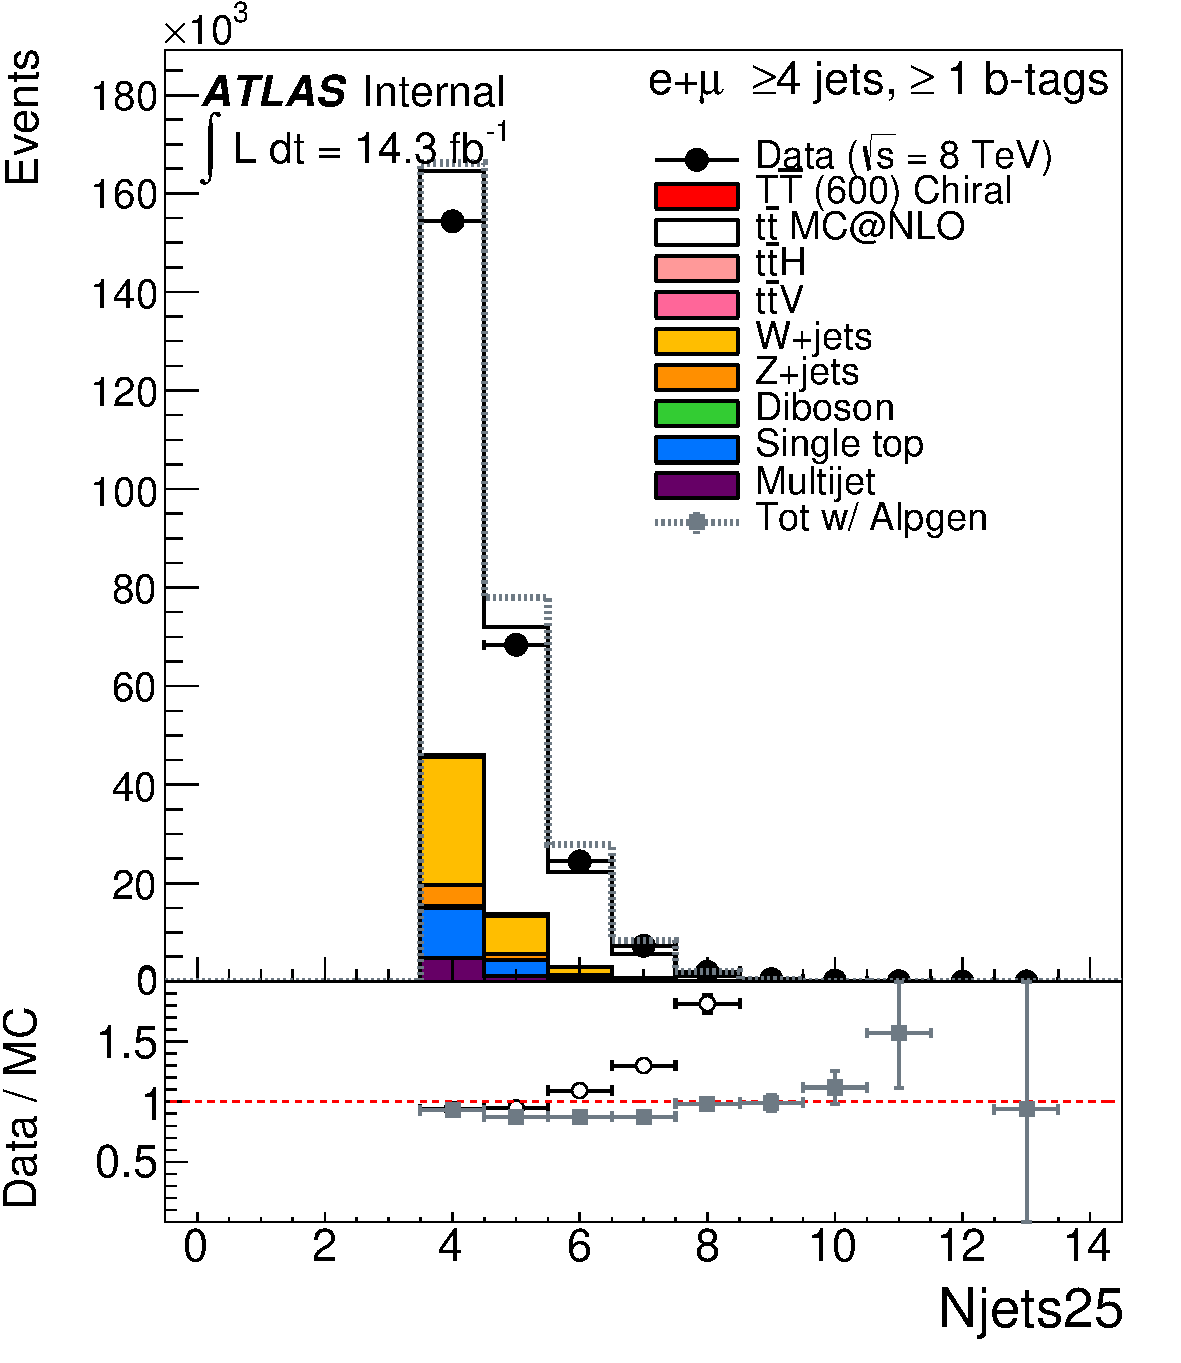
\includegraphics[width=0.29\textwidth]{vlq_analysis/figures/THESIS_c5_presel_noortho_noyields/ELEMUON/4jetin/1btagin/Njets25_ELEMUON_4jetin1btagin_NOMINAL}}
	\subfigure[]{
  	\includegraphics[width=0.29\textwidth]{vlq_analysis/figures/THESIS_c5_presel_noortho_noyields/ELEMUON/4jetin/1btagin/JetPt1_ELEMUON_4jetin1btagin_NOMINAL}}
	\subfigure[]{
  	\includegraphics[width=0.29\textwidth]{vlq_analysis/figures/THESIS_c5_presel_noortho_noyields/ELEMUON/4jetin/1btagin/JetEta1_ELEMUON_4jetin1btagin_NOMINAL}}\\
	\subfigure[]{
  	\includegraphics[width=0.29\textwidth]{vlq_analysis/figures/THESIS_c5_presel_noortho_noyields/ELEMUON/4jetin/1btagin/MET_ELEMUON_4jetin1btagin_NOMINAL}}
	\subfigure[]{
  	\includegraphics[width=0.29\textwidth]{vlq_analysis/figures/THESIS_c5_presel_noortho_noyields/ELEMUON/4jetin/1btagin/LepPt_ELEMUON_4jetin1btagin_NOMINAL}}
	\subfigure[]{
  	\includegraphics[width=0.29\textwidth]{vlq_analysis/figures/THESIS_c5_presel_noortho_noyields/ELEMUON/4jetin/1btagin/LepEta_ELEMUON_4jetin1btagin_NOMINAL}}\\
	\subfigure[]{
  	\includegraphics[width=0.29\textwidth]{vlq_analysis/figures/THESIS_c5_presel_noortho_noyields/ELEMUON/4jetin/1btagin/Wlep_MassT_ELEMUON_4jetin1btagin_NOMINAL}}
	\subfigure[]{
  	\includegraphics[width=0.29\textwidth]{vlq_analysis/figures/THESIS_c5_presel_noortho_noyields/ELEMUON/4jetin/1btagin/HTHad_ELEMUON_4jetin1btagin_NOMINAL}}
	\subfigure[]{
  	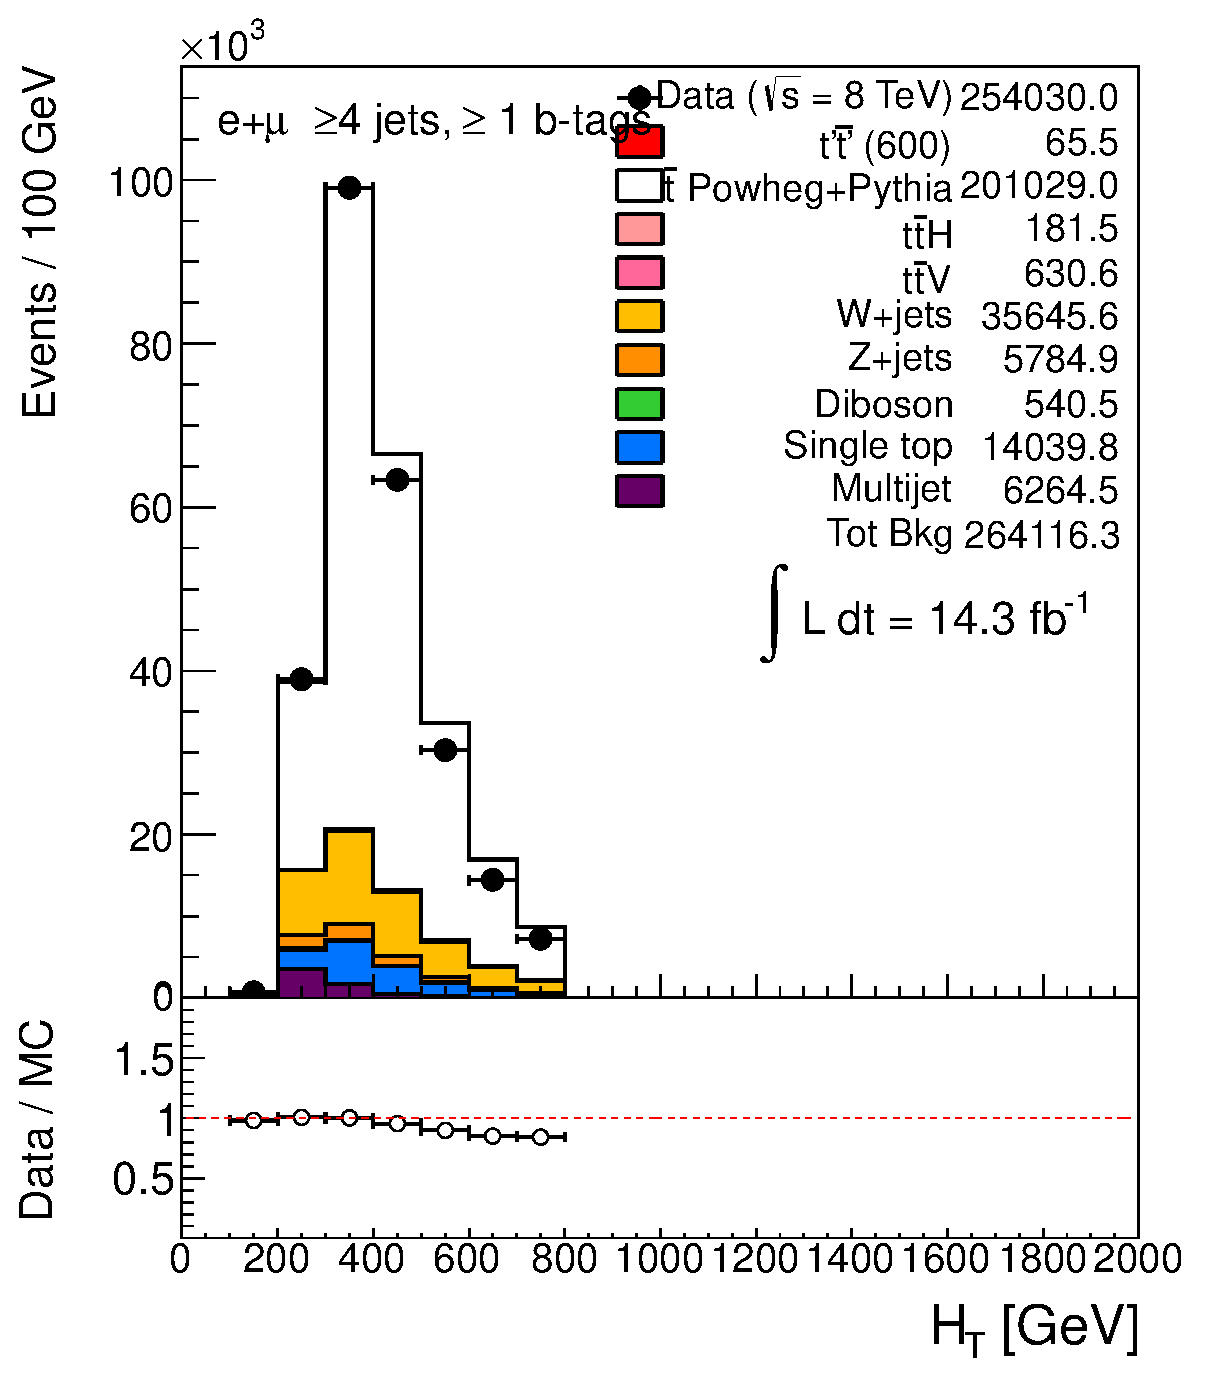
\includegraphics[width=0.29\textwidth]{vlq_analysis/figures/THESIS_c5_presel_noortho_noyields/ELEMUON/4jetin/1btagin/HTAll_ELEMUON_4jetin1btagin_NOMINAL}}
	\caption[]{Comparison between data and prediction in the
        combined electron and muon 
        channel in the blinded control region with at least four jets and
        no \bjet s
        \input{appendices/datamc_variablelist.tex}
	\label{fig:appELEMUON_4jetin1btagin}}
\end{center}\end{figure}

